\subsection{Dữ liệu: Khung tham chiếu - tóm lược}
KronoMiner [488] là một công cụ thăm dò chuỗi thời gian đa năng cung cấp khả năng điều hướng phong phú và hỗ trợ phân tích (hình (\ref{fig:f7.3})). Biễu diễn của nó dựa trên bố cục tâm phân cấp, cho phép người dùng có thể  quan sát chi tiết bằng cách tập trung vào các mảnh khác nhau. Các mảnh dữ liệu có thể được xoay, kéo, co dãn hoặc thu nhỏ một cách dễ dàng, hỗ trợ nhiều kiểu phân tích dữ liệu thời gian. KronoMiner cũng giới thiệu 2 kỹ thuật phân tích: (1) MagicAnalytics Lens, thể hiện mối tương quan của 2 thành phần dữ liệu xếp chồng lên nhau và (2) chế độ Best Match, trong đó một hình cung được hiển thị thể hiện sự tương tự của hai thành phần dữ liệu theo một phép đo cụ thể. 
\begin{figure}[H] % places figure environment here   
    \centering % Centers Graphic
    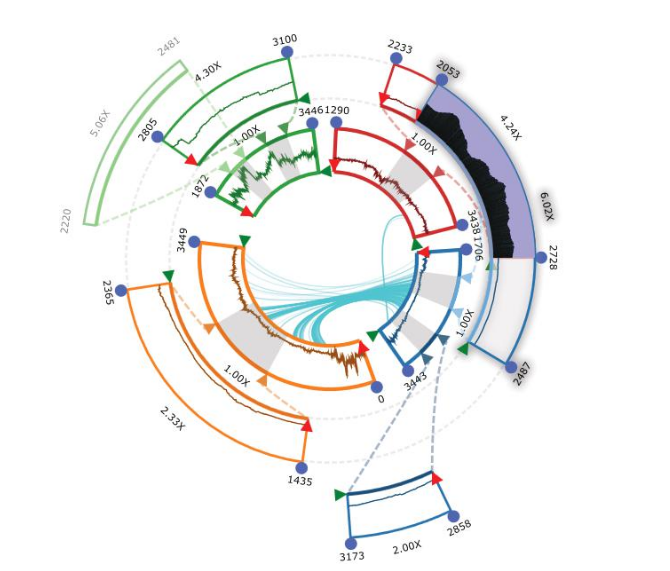
\includegraphics[width=1\textwidth]{assets/fig_7_3.png} 
    \caption{KronoMiner [488]. KronoMiner là một công cụ khám phá chuỗi thời gian đa mục đích cung cấp các tính năng điều hướng và phân tích phong phú} % Creates caption underneath graph
    \label{fig:f7.3}
\end{figure}